%!TEX root = chi14grammatical.tex


Our goal was to find out whether showing examples improves the recognizability of grammatical relations. We tested two types of examples: a list of matching words and a list of matching phrases. Words are explicitly visible in the text, but phrases provides contextual information that helps determine the relationship, such as the part of speech, the relative ordering, and some contextualizing words.

Our hypothesis was:
\begin{quote}
	H1. Participants are more accurate at identifying grammatical relations if shown with examples of contextualizing words or phrases than without.
\end{quote}

To test H1, participants were given a series of identification tasks. In each task, they were shown a list of 8 sentences, each containing a particular relationship between highlighted words. They were asked to identify the relationship from a list of 4 choices.  Additionally, one word was chosen as a \emph{focus word} that was consistent across all examples in that task to make the relationship more recognizable (``life'' in Figure~\ref{fig:choices}).

The choices were displayed in 3 different ways (Figure \ref{fig:choices}).  The \strong{baseline} presentation 
(Figure \ref{fig:baseline-choices}) named the linguistic relation and showed the blank space with a peach background color representing the varying word in the relationship, the focus word that stays constant throughout the task with a yellow background and underlined, and any necessary additional words necessary to convey the relationship (such as "of" for the prepositional relationship containing "of").
 
The \strong{words} presentation showed the baseline design, and in addition beneath it showed the word ``Examples:'' followed by a list of 4 example words that could fill in the peach-colored blank slot (Figure \ref{fig:words-choices}).   The \strong{phrases} presentation again showed the baseline design, beneath which was shown the phrase ``Patterns like:'' and a list of 4 example phrases in which fragments of text including both the peach and the yellow highlighted portions of the  relationship appeared (Figure \ref{fig:task}).

In a between-subjects design the task order and the choice order were not varied: the only variation between participants the presentation design.  
To avoid the possibility of participants guessing the right answer by pattern-matching, we ensured that there was no overlap between the list of sentences shown, and the examples shown in the choices as words or phrases. Not every relationship shown in the distractors was tested, and distractors were chosen to be ones intuitively most likely to be mistaken for  the relationship shown.

The tasks were generated using the Stanford Dependency Parser \cite{de2006generating} on the text of \emph{Moby Dick} by Herman Melville.  We tested the 12 most common grammatical relationships in the novel, which fell into two categories:.

\squishlist
\item Clausal or long-distance relations:
	\squishlist
		\item \strong{advcl} Adverbial clause: \emph{  she \textbf{said} it while \textbf{smiling}}
		\item  \strong{xcomp} Open clausal complement:  \emph{I \textbf{learned} to \textbf{sing} }
		\item  \strong{ccomp} Clausal complement:  \emph{ I \textbf{thought} that I \textbf{knew} it}
		\item  \strong{rcmod} Relative clause modifier:  \emph{the \textbf{cat}, which we \textbf{rescued}, slept }
	\squishend
\item Other relations:
		\squishlist
			\item \strong{nsubj} Subject of verb: \emph{\textbf{he} \textbf{threw} the ball}
			\item \strong{dobj} Object of verb:  \emph{ he \textbf{threw} the \textbf{ball}}
			\item \strong{amod} Adjective modifier \emph{\textbf{red} \textbf{ball}}
			\item \strong{prep\_in}  Preposition (in): \emph{ the \textbf{water} in the \textbf{bucket}}
			\item \strong{prep\_of}	Preposition (of):  \emph{ the \textbf{piece} of \textbf{cheese}}
			\item \strong{conj\_and}  Conjunction (and)  \emph{ \textbf{mind} and \textbf{body}}
		\item\strong{advmod} Adverbial modifier: \emph{  she \textbf{said} it \textbf{slowly}}
		\item \strong{nn} Noun compound:  \emph{ \textbf{Mr.}  \textbf{Brown}}
		\squishend
\squishend

We tested each of the above relations 4 times, with 2 different words in each role. For example, the verb-subject relation \code{nsubj} was tested in the following forms:
\squishlist
	\item \code{nsubj(Ahab, \_\_\_)}:  the sentences each contained `Ahab', highlighted in yellow, as the subject of different verbs highlighted in peach.
	\item \code{nsubj(captain, \_\_\_)}

	\item \code{nsubj(\_\_\_, said)}: the sentences all contained the verb `said', highlighted in yellow, but with different subjects, highlighted in peach.
	\item \code{nsubj(\_\_\_, stood)}
\squishend

To maximize coverage, yet keep the total task time reasonable (average XX minutes), we divided the relations above into 4 task sets of 3 relations each. Each relation was tested with 4 different words, making a total of 12 tasks per participant.

\subsection{Participants}
We chose Amazon's Mechanical Turk (MTurk) crowdsourcing platform as a source of study participants.  Since our goal is to find a representation that is understandable to most people, not just linguistic experts, the wide range of backgrounds provided by MTurk is desirable.
Participants were paid 50c (U.S.) for completing the task, with an additional 50c bonus if they correctly identified 10 or more of the 12 relationships. They were informed of the possibility of the bonus before starting the task.  

To help ensure the quality of effort from participants, we included a multiple-choice screening question, `What is the third word of this sentence?"  Those that answered incorrectly were eliminated. 400 participants completed the study distributed randomly over the 4 task sets and the 3 presentations. XXX percent responded positively to a question about syntactic familiarity XXX.


\subsection{Results}
\begin{figure}
\centering
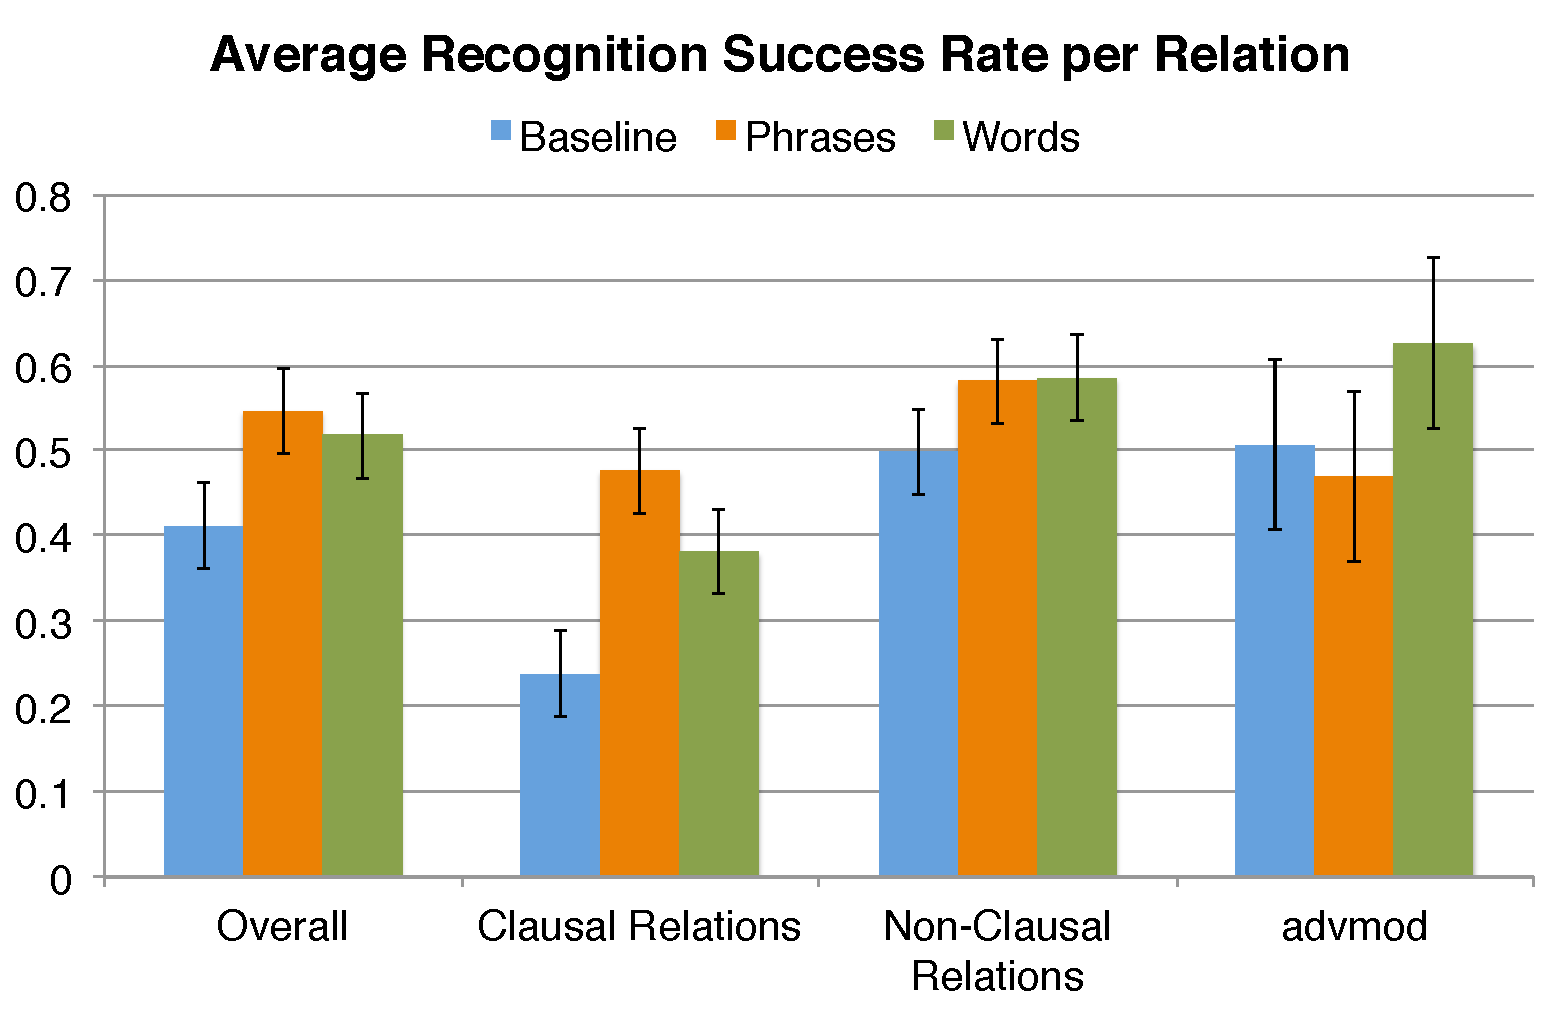
\includegraphics[width=\columnwidth]{fig/results}
\caption{\label{fig:results}Recognition rates per relation group under the different experiment conditions.}
\end{figure}
The results (Figure \ref{fig:results}) confirm H1. Participants in conditions that showed examples (\strong{phrases} and \strong{words}) were significantly better at identifying the relations than participants in the \strong{baseline} condition.  The average success rate (where success means that the participant correctly identified the relation) in the \strong{baseline} condition was $41\%$, which is significantly\footnote{Using the Wilcoxson signed-rank test, an alternative to the standard T-test that does not assume samples are normally distributed.} less accurate than in the two example-showing conditions: \strong{words}: $52\%, (p = 0.00019)$, and \strong{phrases} condition: $55\%, (p = 0.00013)$.

For the clausal relations, which operate over longer distances in sentences, the data confirmed what one might intuitively expect. Phrases, which show the usage context, significantly improved recognizability compared to the list of words or the baseline labels. The average success rate is 48\% for \strong{phrases}, which is significantly more than \strong{words}: 38\%, (p = 0.017), or \strong{baseline}: 24\%, ($p= 1.9 \times 10^9$).

For the non-clausal relations, there was no significant difference between \strong{phrases} and \strong{words}, although they were both overall significantly better than the baseline (words: $p=0.0063$, phrases: $p=0.023$). (XXX this p-value does not look significant XXX) Among these relations, adverb modifiers (\code{advmod}) stood out (Figure \ref{fig:results}), because \strong{words} (0.63\% success) made the relation more recognizable than \strong{phrases} (0.47\% success, $p = 0.055$) -- but the difference was barely significant, due to the smaller sample size (only 96 participants encountered this relation). This may be because the words are the most salient piece of information in an adverbial relation -- adverbs usually end in `ly' -- and in the phrases condition the additional information distracts from recognition of this pattern.

